%% 歩容パターンの再評価手法の提案.tex
%% LaTeX-2e 専用

%% 全体の流れとしては,まず,先行研究の問題点を指摘し,次に,歩容パターンの再評価手法を提案する.

\chapter{歩容パターンの再評価手法の提案}\label{chapter:歩容パターンの再評価手法の提案}
第\ref{chapter:歩容パターンの再評価手法の提案}章では,先行研究の手法およびその問題点を指摘し,
常に脚軌道生成が可能な自由歩容パターン生成手法として,歩容パターンの再評価手法を述べる.

% 先行研究の章
\section{本研究室における自由歩容パターン生成の先行研究}
\subsection{グラフ理論について}
本論文ではグラフ理論を用いた自由歩容パターン生成手法を論ずるため,まずはグラフ理論について述べる.
グラフとは,頂点(ノード)とそれらを結ぶ辺(エッジ)からなる図形である.
このグラフを用いて,さまざまな問題を取り扱う学問をグラフ理論という.

以降の説明を簡単にするため,この論文で用いるグラフ理論の用語について簡潔に述べる.
エッジに向きがあるものを有向グラフ,逆に向きを持たないものを無向グラフという.
また,閉路を持たず,かつ,すべての頂点間に経路が存在するグラフを木という.
このような木構造をもつグラフのうち,図\ref*{fig:tree_graph}のように,
根となるノードを持ち,そのノードからすべてのノードに到達可能なものを根付き木という.

根付き木において,あるノードから遷移可能なノードをそのノードの子ノードと呼ぶ.
逆に,あるノードに遷移可能なノードをそのノードの親ノードと呼ぶ.
親ノードを持たないノードを根ノードと呼び,子ノードを持たないノードを葉ノードと呼ぶ.
また,あるノードから根ノードまでのエッジの数をそのノードの深さと呼び,
根ノード自身の深さは0となる.

図\ref*{fig:tree_graph}においては,ノードAが根ノードであり,ノードB,Cがその子ノードである.
また,ノードB,ノードD,E,ノードCはノードFを子ノードとして持ち,ノードD,E,Fは葉ノードである.
ノードAの深さは0であり,ノードB,Cの深さは1,ノードD,E,Fの深さは2となる.

グラフのあるノードから別のノードに到達するための経路をパスと呼び,
これを求めることをグラフ探索と呼ぶ.
グラフ探索には,深さ優先探索,幅優先探索などのさまざまなアルゴリズムが存在する.
深さ優先探索では,始点となるノードから,深さが深くなる方向を優先して探索を行う.
これに対して,幅優先探索では,始点となるノードから,深さが浅いノードを優先して探索を行う手法である.

\begin{figure}[tbp]
  \begin{center}
    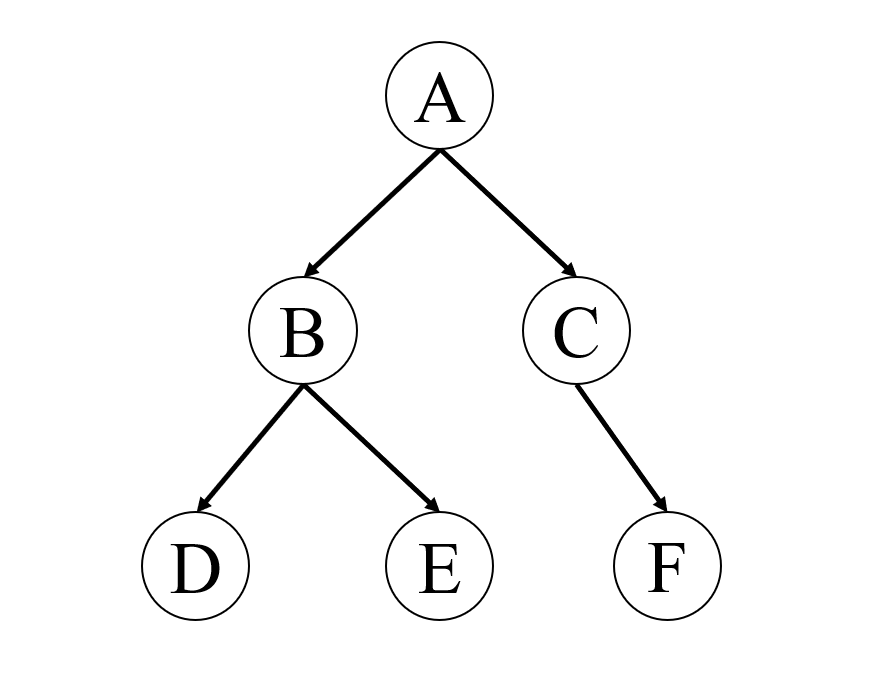
\includegraphics[width=50mm, clip]{figure/tree_graph.png}
   \caption{Tree Graph}
   \label{fig:tree_graph}
  \end{center}
\end{figure}

\subsection{歩容パターングラフの定義}
本研究においては,6脚ロボットの歩容パターンをグラフを用いて表現する.
これは,ロボットの状態をノードとし,ロボットの状態間の遷移,つまりロボットの動作をエッジとしてグラフを作成する.
グラフは有向の根付き木とし,現在のロボットの状態を根ノード,その姿勢から1動作で到達できる姿勢を子ノードとして根ノードに接続する.
また,このようにして作られたグラフを歩容パターングラフと定義する.

グラフ探索がよく用いられる題材は路線図や回路図などであり,ノードの数が有限である.
しかし,歩容パターングラフはロボットの状態や動作を対象とするため,無数の組み合わせが存在する.
そのため,先行研究では状態や動作を離散化することで歩容パターン生成をグラフへ落とし込んでいる.
以下に各要素の離散化について述べる.

\subsubsection{脚位置の離散化}

\subsubsection{グラフの階層構造}

\subsubsection{エッジの離散化}
エッジの離散化について述べる.
前述したように歩容パターングラフにおいて,エッジはロボットの動作を表す.
ロボットの動作は,脚の接地・遊脚運動と,重心の移動からなる.

\subsubsection{脚軌道生成の分離}
これまで離散化された脚位置やその遷移について論じてきたが,実際に脚を動作させるためには脚軌道について考える必要がある.
これは,脚軌道生成をグラフ探索による歩容パターン生成から分離しているためである.
歩容パターン生成に脚軌道生成を組み込んだ場合,

\subsection{脚軌道生成の失敗}


% 予備実験の章
\section{歩行シミュレーションによる脚軌道生成失敗時の脚先位置の特定}

\subsection{シミュレーション実験の目的}
先行研究では脚軌道生成の失敗による動作の停止が報告された上,その原因は脚先が脚の可動範囲の外を通ることによるものであると考察されてきた.
しかし,具体的に脚先がどのような位置になると脚軌道生成が失敗するのかは明らかにされていなかった.
そのため予備実験として,先行研究と同じ条件で歩行シミュレーション実験を行い,ロボットの脚軌道を確認することで,脚軌道生成失敗の原因を考察した.

\subsection{シミュレーションの条件}
本研究室ではロボットの動作のシミュレーションを行うためのシミュレーターソフトウェアを自作し,シミュレーション実験で用いてきた.
シミュレーターはC++で記述されており,WindowsAPIを用いてGUIを実装し,ロボットを表示している.
また,GUIの表示のプログラムをより簡単に記述するため,ゲームプログラミングに用いられるライブラリのDxLibを用いている.

シミュレーターは物理演算を行っておらず,トルク不足や摩擦,脚先の滑りによるずれを考慮していない.
そのため,ロボットのアクチュエータは無限のトルクを持ち,脚先は滑りなく接地するものと仮定している.
本来これらのパラメータを考慮すべきではあるが,本研究においては歩容パターン生成が可能であるかを確認することが目的であるため,これらのパラメータは考慮しないこととしている.

\subsection{シミュレーションの結果}
以下の図に脚軌道生成失敗時の脚先の座標を示す.

\subsection{脚軌道生成の失敗の原因の考察}

\section{常に脚軌道生成が可能な自由歩容パターン生成手法の検討}
常に脚軌道生成を可能にするためには,近似された脚可動範囲を適切に設定する必要がある.


\section{歩容パターンの再評価手法}

